\documentclass[10pt]{article}
\usepackage[utf8]{inputenc}
\usepackage{amsthm}
\usepackage{amsmath, mathtools, amsfonts,amssymb}
\usepackage{graphicx}
\usepackage{verbatim}
\usepackage{fancyhdr}
% Code
\usepackage{listings}
\usepackage{algorithm}
\usepackage{algpseudocode}
% Margins
\usepackage{geometry}
%\usepackage{enumitem} % for nice enumerating
\geometry{margin=0.75in}
\usepackage{verbatim} % what is this for again???
\usepackage{tcolorbox}
\usepackage[symbol]{footmisc}
% Graphics
\usepackage{caption} % Nice captions
\usepackage{tikz}
\usetikzlibrary{matrix} % matrices
\usepackage{tikz-qtree} % Simple trees
\usetikzlibrary{positioning}
\tikzset{main node/.style={circle, draw,minimum size=0.5cm,inner sep=0pt},
}
\tikzset{other node/.style={minimum size=0.5cm,inner sep=0pt},
}
\tikzset{blue node/.style={circle, draw,minimum size=0.5cm,inner sep=0pt, color
    = blue},
}
\tikzset{red node/.style={circle, draw,minimum size=0.5cm,inner sep=0pt, color
    = red},
}
\tikzset{teal node/.style={circle, draw,minimum size=0.5cm,inner sep=0pt, color
    = teal},
}
\tikzset{red node/.style={circle, draw,minimum size=0.5cm,inner sep=0pt, color
    = red},
}
\tikzset{magenta node/.style={circle, draw,minimum size=0.5cm,inner sep=0pt, color
    = magenta},
}
\tikzset{orange node/.style={circle, draw,minimum size=0.5cm,inner sep=0pt, color
    = orange},
}
\tikzset{violet node/.style={circle, draw,minimum size=0.5cm,inner sep=0pt, color
    = violet},
}
\tikzset{yellow node/.style={circle, draw,minimum size=0.5cm,inner sep=0pt, color
    = yellow},
}
\setcounter{section}{-1}
\usepackage{mathrsfs}
\newtheorem{pic}{Figure}
\numberwithin{pic}{section}
\newtheorem{lem}{Lemma}
\numberwithin{lem}{section}
\newtheorem{thm}{Theorem}
\numberwithin{thm}{section}
\newtheorem{cor}{Corollary}
\numberwithin{cor}{section}

\theoremstyle{definition}
\newtheorem{ex}{Example}
\numberwithin{ex}{section}
\newtheorem{defn}{Definition}
\numberwithin{defn}{section}
\theoremstyle{definition}
\newtheorem{prob}{Problem}
\numberwithin{prob}{section}
\theoremstyle{remark}
\newtheorem*{con}{Conjecture}
\newtheorem*{rem}{Remark}
\newtheorem*{cex}{Counterexample}
\newtheorem*{ts}{T.S.}
\theoremstyle{plain}
\newtheorem{claim}{Claim}
\numberwithin{claim}{prob}
%%% COMMANDS %%%
% Sets
\newcommand{\set}[1]{\ensuremath{\left\{ #1\right\}}} % write sets
\newcommand{\e}{\ensuremath{\epsilon}} % Epsilon
\newcommand{\R}{\ensuremath{\mathbb{R}}} % Real Numbers
\newcommand{\N}{\ensuremath{\mathbb{N}}} % Natural numbers
\newcommand{\Q}{\ensuremath{\mathbb{Q}}} % Rationals
\newcommand{\I}{\ensuremath{\mathbb{I}}} % Irrational Numbers
\newcommand{\Z}{\ensuremath{\mathbb{Z}}} % Integers
% Probability
\newcommand{\Prob}{\ensuremath{\mathbb{P}}} % Probability
\newcommand{\Ex}{\ensuremath{\mathbb{E}}} % Expected Value
\newcommand{\var}{\ensuremath{\text{Var}}} % Variance
\newcommand{\cov}{\ensuremath{\text{Cov}}} % Covariance
% Easier Delimiters?
\newcommand{\lr}[2]{\ensuremath{\left#1 #2 \right #1}}
% Absolute Value
\newcommand{\abs}[1]{\ensuremath{\left| #1 \right|}}
% Landau Notation
\newcommand{\Oh}{\ensuremath{\mathcal{O}}} %%% IN MATH MODE
% Display style fractions
\newcommand{\Frac}[2]{\displaystyle \frac{#1}{#2}}
% Display style limits
\newcommand{\Lim}[2]{\displaystyle \lim_{#1}{#2}}

% Enumerate
\renewcommand{\labelenumi}{(\alph{enumi})}
\renewcommand{\labelenumii}{\roman{enumii}}

% change proof environment
%\renewcommand*{\proofname}{Pf}

% Line Spacing
\renewcommand{\baselinestretch}{1.5}

% Indentation
\newlength\tindent
\setlength{\tindent}{\parindent}
\setlength{\parindent}{0pt}
\renewcommand{\indent}{\hspace*{\tindent}}
\renewcommand\qedsymbol{{$\blacksquare$}}
% Set title
\title{X}

\begin{document}


\tcbset{colback=white, sharp corners, leftrule=0.2mm, toprule=0.2mm,
  bottomrule=0.2mm, rightrule=0.2mm} % Options for boxes
\fancyhead[l]{Nate CS Practice}
\fancyhead[c]{Assignment I}
\fancyhead[r]{\today}
\pagestyle{fancy}

\section{Math Exercises}
\begin{prob}
  DeMorgan's laws state that
  \begin{align}
    \neg(P \vee Q) &\iff \neg P \wedge \neg Q\\
    \neg(P \wedge Q) &\iff \neg P \vee \neg Q
  \end{align}
  Prove one of these identities by way of a truth table.
\end{prob}
\begin{prob}
  Consider the following recursively defined function,
  $$f(n) =
  \begin{cases}
    1 &\text{if }n \leq 1\\
    n\cdot f(n / 2) &\text{if }n\mod 2 = 0\\
    n + f(n - 1) &\text{if }n\mod 2 = 1
  \end{cases} $$
  Calculate $f(20)$.
\end{prob}
\begin{prob}
  Let $a,b$ be characters, $\epsilon$ be the empty string, and $\circ$ denote string concatenation. Consider the following definition of a $foo$,
  $$foo =
  \begin{cases}
    \epsilon\\
    a\circ foo \circ a\\
    a\circ foo \circ b\\
    b\circ foo \circ a\\
    b\circ foo \circ b
  \end{cases}
  $$
  \begin{enumerate}
  \item Is $aba$ a $foo$?
  \item Is $babb$ a $foo$?
  \item In more intuitive terms, what is a $foo$?
  \end{enumerate}
\end{prob}
\begin{prob}
  A \textit{Triangular Number} counts objects that are arranged into equilateral triangles (see the image below, lifted from Wikipedia).\\
  \begin{center}
    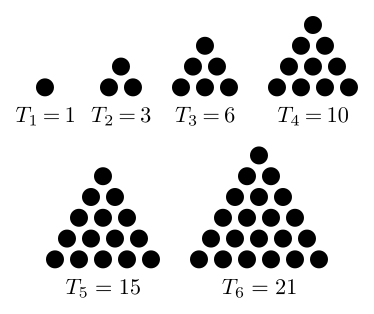
\includegraphics[scale=0.5]{TriNums}
  \end{center}
  \begin{enumerate}
  \item Come up with a recursive definition for $T_n$, the $n^{th}$ triangular number.
  \item Come up with a non-recursive formula for $T_n$ (extra credit: prove this formula via induction).
  \item Let $S_n$ denote the sequence of non-zero perfect squares, i.e. $S_1 =
    1, S_2 = 4, S_3 = 9, ...$. Prove that $S_n = T_n + T_{n-1}$ for $n \geq 2$.
    \textit{Hint:} the closed formula from part (b) may be helpful.It may also
    help to try devising a ``proof by picture'' first.
  \end{enumerate}
\end{prob}
\section{Computer Problems}
\begin{center}
  All problems from this section should be uploaded to \texttt{Github}
\end{center}

\begin{comment}
\begin{prob}
  Write a \textit{C} program to read in a number, and then display some silly math facts about that number, i.e. $x$ times 7 is $y$, $x^2$ is $z$, etc. Add this program to github.
\end{prob}
\end{comment}
\begin{prob}
  Write a \textit{C} program that takes in two integers and outputs the division algorithm performed with those two numbers as inputs. Below is an example of output.\\
  \begin{center}
    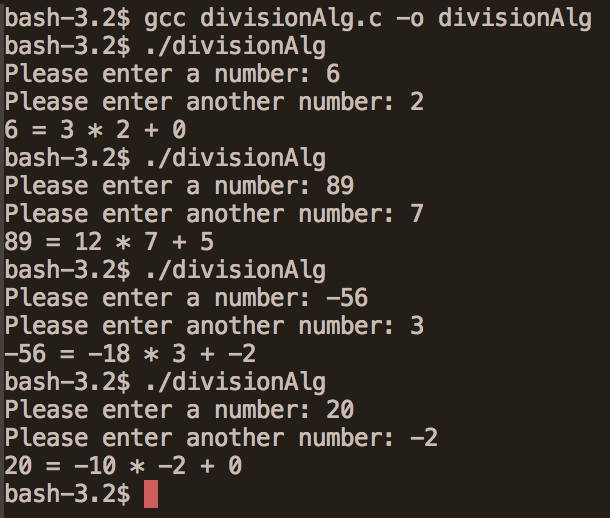
\includegraphics[scale=0.5]{soln1}
  \end{center}
\end{prob}
  \begin{prob}[Quadratic Formula] Write a \texttt{C} program that takes as input
    three real numbers $a,b,c$ which determine a quadratic equation of the form
    \begin{equation*}
      ax^2 + bx + c = 0,
    \end{equation*}
    and outputs any real roots of that equation. Your program should determine
    whether your equation has zero, one, or two real roots, and indicate this to
    the user (you do not need to compute complex roots).
  \end{prob}
\end{document}